\section{CALCE dataset and preprocessing}
\subsection{Dataset description}
Four Excel files of cell SP20-1 were audited (\texttt{docs/DATASET\_AUDIT\_REPORT.md}). Each 0.1\,A test follows: rest (2\,h), constant-current discharge to 2.5\,V, rest (2\,h), constant-current charge, rest. The initial-capacity test uses 1\,A with a constant-voltage phase (Fig.~\ref{fig:raw}). Temperatures 0/25/45\,°C are taken from file names; a single 23\,°C reading exists in the 25\,°C file and the 1\,A file carries no temperature. The files use different schemas (Arbin full export vs.\ reduced export in mV/mA), event-driven vs.\ 1\,s logging, and the 0\,°C file is an OOXML workbook with a \texttt{.xls} extension; the loader is configuration-driven (\texttt{configs/dataset\_config.yaml}).
\begin{figure}[H]\centering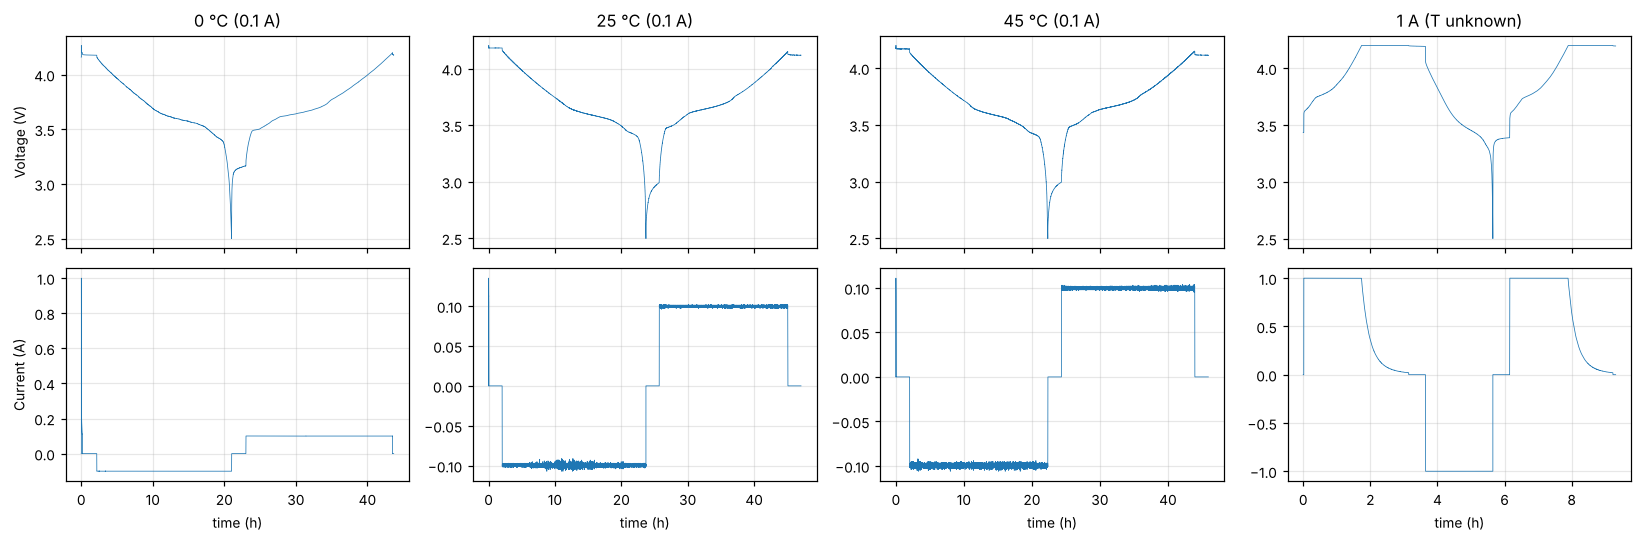
\includegraphics[width=\linewidth]{fig01_raw_overview.png}\caption{Measured voltage and current of the four tests.}\label{fig:raw}\end{figure}
\paragraph{Findings constraining the study.} (1) One cycle per file (no ageing); (2) one cell; (3) no usable temperature measurement; (4) no documented nominal capacity; (5) no measured SOC; (6) 25/45\,°C charge phases stop near 4.15\,V. Table~\ref{tab:capacity} lists measured delivered capacities; the lower value at 45\,°C than at 25\,°C is unexpected and is confounded with test history (tests span Oct.\ 2015--Feb.\ 2016).
\begin{table}[htbp]\centering\footnotesize
\begin{tabular}{lrrrr}
\toprule
 & Mean I (A) & Delivered Q (Ah) & Q / Q$_{25}$ (\%) & R$_0$ ($\Omega$) \\
Condition &  &  &  &  \\
\midrule
0\,°C & -0.100 & 1.882 & 87.240 & 0.132 \\
25\,°C & -0.100 & 2.157 & 100.000 & 0.080 \\
45\,°C & -0.100 & 2.022 & 93.750 & 0.082 \\
1\,A & -1.000 & 2.009 & 93.150 & 0.126 \\
\bottomrule
\end{tabular}
\caption{Measured delivered capacity (2.5\,V cut-off) and R$_0$ at discharge onset per test. Temperatures are file-name labels. These are not SOH values.}\label{tab:capacity}
\end{table}


\subsection{Preprocessing}
The pipeline performs unit conversion, duplicate-timestamp removal, physical-range checks, charge/discharge/rest segmentation from the current sign (20\,mA tolerance, 10\,min minimum), and linear resampling to a 20\,s grid. Features are limited to quantities that exist in all files: voltage, current, a causal 10\,min voltage moving average and a 10\,min voltage difference. Energy, internal-resistance and temperature statistics are not used because they are not available in every file.
